\documentclass{elsarticle_nonatbib}\usepackage[]{graphicx}\usepackage[]{color}
%% maxwidth is the original width if it is less than linewidth
%% otherwise use linewidth (to make sure the graphics do not exceed the margin)
\makeatletter
\def\maxwidth{ %
  \ifdim\Gin@nat@width>\linewidth
    \linewidth
  \else
    \Gin@nat@width
  \fi
}
\makeatother

\definecolor{fgcolor}{rgb}{0.345, 0.345, 0.345}
\newcommand{\hlnum}[1]{\textcolor[rgb]{0.686,0.059,0.569}{#1}}%
\newcommand{\hlstr}[1]{\textcolor[rgb]{0.192,0.494,0.8}{#1}}%
\newcommand{\hlcom}[1]{\textcolor[rgb]{0.678,0.584,0.686}{\textit{#1}}}%
\newcommand{\hlopt}[1]{\textcolor[rgb]{0,0,0}{#1}}%
\newcommand{\hlstd}[1]{\textcolor[rgb]{0.345,0.345,0.345}{#1}}%
\newcommand{\hlkwa}[1]{\textcolor[rgb]{0.161,0.373,0.58}{\textbf{#1}}}%
\newcommand{\hlkwb}[1]{\textcolor[rgb]{0.69,0.353,0.396}{#1}}%
\newcommand{\hlkwc}[1]{\textcolor[rgb]{0.333,0.667,0.333}{#1}}%
\newcommand{\hlkwd}[1]{\textcolor[rgb]{0.737,0.353,0.396}{\textbf{#1}}}%

\usepackage{framed}
\makeatletter
\newenvironment{kframe}{%
 \def\at@end@of@kframe{}%
 \ifinner\ifhmode%
  \def\at@end@of@kframe{\end{minipage}}%
  \begin{minipage}{\columnwidth}%
 \fi\fi%
 \def\FrameCommand##1{\hskip\@totalleftmargin \hskip-\fboxsep
 \colorbox{shadecolor}{##1}\hskip-\fboxsep
     % There is no \\@totalrightmargin, so:
     \hskip-\linewidth \hskip-\@totalleftmargin \hskip\columnwidth}%
 \MakeFramed {\advance\hsize-\width
   \@totalleftmargin\z@ \linewidth\hsize
   \@setminipage}}%
 {\par\unskip\endMakeFramed%
 \at@end@of@kframe}
\makeatother

\definecolor{shadecolor}{rgb}{.97, .97, .97}
\definecolor{messagecolor}{rgb}{0, 0, 0}
\definecolor{warningcolor}{rgb}{1, 0, 1}
\definecolor{errorcolor}{rgb}{1, 0, 0}
\newenvironment{knitrout}{}{} % an empty environment to be redefined in TeX

\usepackage{alltt}
\usepackage[top=1in, left=1in, right=1in, bottom=1in]{geometry}

\usepackage{float, amsmath}
\usepackage{tikz}
\usetikzlibrary{shapes,arrows}
\usetikzlibrary{positioning}
\usepackage{float, amsmath}

\usepackage[hyphens]{url}
\usepackage{enumerate}
%\usepackage{chapterbib}
% \usepackage{natbib}
\usepackage{setspace} % delete when  \singlespacing is taken out 


\usepackage[
  natbib = true,
    backend=bibtex,
    isbn=false,
    url=false,
    doi=false,
    eprint=false,
    style=numeric,
    sorting=nyt,
    sortcites = true
]{biblatex}
\bibliography{CT_Skull_Stripping_Bib}
\bibliography{CT_ICH_Segmentation}
\bibliography{extra_bibs_addon}
\AtEveryBibitem{
\clearfield{note}
% \clearlist{address}
% \clearfield{eprint}
% \clearfield{isbn}
% \clearfield{issn}
% \clearlist{location}
% \clearfield{month}
% \clearfield{series}
} % clears language

\usepackage{hyperref}

\makeatletter
\providecommand{\doi}[1]{%
  \begingroup
    \let\bibinfo\@secondoftwo
    \urlstyle{rm}%
    \href{http://dx.doi.org/#1}{%
      doi:\discretionary{}{}{}%
      \nolinkurl{#1}%
    }%
  \endgroup
}
\makeatother

\newcommand{\pkg}[1]{\texttt{#1}}
\newcommand{\code}[1]{\texttt{#1}}

\usepackage{subfig}

\journal{NeuroImage}









%\usepackage[all]{hypcap}
\IfFileExists{upquote.sty}{\usepackage{upquote}}{}
\begin{document}
\renewcommand{\thesubfigure}{\Alph{subfigure}}

\begin{frontmatter}

\date{}

\title{PItcHPERFECT: Primary Intracranial Hemorrhage Probability Estimation using Regression and Features Extracted from CT}
%\title{Validated Automatic Brain Extraction of Head CT Images using Established, Open-Source, Neuroimaging Software}



\auth[jhsph]{John~Muschelli\corref{cor1}}
\ead{jmusche1@jhu.edu}

\auth[jhsph]{Elizabeth~M.~Sweeney}
\ead{emsweene1@jhu.edu}

\auth[ucla]{Paul~Vespa}
\ead{PVespa@mednet.ucla.edu}

\auth[jhmi]{Daniel~F.~Hanley}
\ead{dhanley@jhmi.edu}

\auth[jhsph]{Ciprian~M.~Crainiceanu}
\ead{ccrainic@jhsph.edu}


\cortext[cor1]{Principal Corresponding Author}
\address[jhsph]{Department of Biostatistics, Bloomberg School of Public Health, Johns Hopkins University, Baltimore, MD, USA}
\address[jhmi]{Department of Neurology, Division of Brain Injury Outcomes,  Johns Hopkins Medical Institutions, Baltimore, MD, USA}
\address[ucla]{Department of Neurosurgery, David Geffen School of Medicine at UCLA, Los Angeles, CA, USA}


\begin{abstract}

%
%\section*{Introduction}
%Intracerebral hemorrhage (ICH) is a neurological condition that results from a blood vessel rupturing into the tissue and possibly the ventricles of the brain; it accounts for approximately 10-15\% of all strokes and 5 million cases worldwide \citep{krishnamurthi_global_2014}. 
%
%Manual segmentation using planimetry is the gold standard for volume estimation but is time-consuming and has within- and across-reader variability.  We wish to create an algorithm that can estimate the probability of ICH at a voxel-level, the volume of ICH, and the level of uncertainty in these estimates.  We propose an automated segmentation using logistic regression with features extracted from X-ray computed tomography (CT) scans.  
%\vspace{-1em}
%\section*{Data}
%The Minimally Invasive Surgery and rt-PA in ICH Evacuation (MISTIE) trial was a multi-site, multi-national, randomized Phase II clinical trial. We used 112 patients from MISTIE, one scan per patient, using the first scan acquired, for model estimation and validation.  
%\vspace{-1em}
%\subsection*{Manual ICH Segmentation}
%ICH was manually segmented on CT scans by expert readers. Binary hemorrhage masks were created by setting voxel intensity to $1$ if the voxel was classified as hemorrhage, regardless of location, and $0$ otherwise.  CT images were preprocessed and brains were extracted using a validated CT-specific brain extraction protocol \citep{muschelli_iii_validated_2015}, and eroded.  We derived a set of imaging predictors from each scan.  We used the first $10$ scans as a training set: we aggregated voxels, performed a voxel selection procedure and fit the model: 
%$$\mbox{logit}(Y(v)) = \alpha + X(v) \beta$$
%where $X(v)$ is a set of features for voxel $v$ and $Y(v)$ is the binary presence of ICH.  We validated this model on another $51$ scans: we estimated the probability a voxel is ICH, and thresholded the probability to give a binary prediction. We used the Dice Similarity Index (DSI) \citep{dice_measures_1945} to estimate performance where $DSI = \frac{2 \times \text{TP} }{ 2\times \text{TP} + \text{FN} + \text{FP}}$, which ranges from $0$ to $1$, where TN/TP are true negatives/positives, and FN/FP are false negatives/positives, respectively.
%
%\section*{Results} 
%
%The mean (SD) DSI was $0.861$ ($0.052$) for the $51$ validation scans had a high, with a minimum DSI of $0.686$.   These results indicate that the approach described can achieve accurate segmentation of ICH in a population of patients from a variety of imaging centers.  
%
%\vspace{-1em}
%\section*{Future Work}
%Although we have shown the ability to segment hemorrhage well on a number of CT scans, there is room for improvement in the algorithm.  Many of the covariates likely represent redundant or non-orthogonal information.  We can drop groups of variables to detect which are important for accurate prediction at the population level. We must also compare our results to those previously published.


\end{abstract}

\begin{keyword}
CT \sep ICH Segmentation
\end{keyword}

\end{frontmatter}




\section{Introduction}


%Bleeding may cause distension of the brain structures an increase in potentially lethal intracranial pressure (ICP).  ICH is a serious condition; it accounts for approximately 10-15\% of all strokes, corresponding to an estimated 79,500 annual cases \citep{go_heart_2013} and approximately 30,000 deaths \citep{qureshi_spontaneous_2001} in the US and approximately 5 million cases worldwide \citep{krishnamurthi_global_2014}. In addition to the increased likelihood of death, ICH has debilitating health effects on survivors who do not have full functional recovery after stroke.

Intracerebral hemorrhage (ICH) is a neurological condition that results from a blood vessel rupturing into the tissue and possibly the ventricles of the brain.   The use of X-ray computed tomography (CT) scans allows clinicians and researchers to qualitatively and quantitatively describe the characteristics of a hemorrhage to guide interventions and treatments.  CT scanning is widely available and is the most commonly used diagnostic tool in patients with ICH \citep{sahni_management_2007}.  The volume of ICH has been consistently demonstrated to be an important diagnostic predictor of stroke severity, long-term functional outcome, and mortality \citep{broderick_volume_1993, hemphill_ich_2001, tuhrim_volume_1999}.  ICH volume change is also common primary outcome \citep{anderson_intensive_2008, anderson_effects_2010, qureshi_association_2011, mayer_recombinant_2005} and secondary outcome \citep{morgan_preliminary_2008_mistie, anderson_intensive_2008, morgan_preliminary_2008_clear} in clinical trials.  Moreover, the location of the ICH has been shown to affect functional outcome in patients with stroke \citep{rost_prediction_2008, castellanos_predictors_2005}.

ICH volume can be rapidly measured using techniques such as the ABC/2 method \citep{broderick_volume_1993}.  In this method, a reader chooses which slice has the largest area of hemorrhage, draws a line along the longest axis of the hemorrhage (denoted A) and the orthogonal line that bisects the hemorrhage (B).  The reader then counts the number of slices where hemorrhage is present (C).  The volume estimate is $\frac{A\times B\times C}{2}$, which is an approximation of an ellipsoid \citep{kothari_abcs_1996}.  As this method only requires 3 measurements, this method can be done rapidly. 

Although ABC/2 is is widely used, \citet{divani_abcs_2011} found that volume measurement errors using ABC/2 were significantly greater than those using planimetry measurements at measuring the true volume of a hemorrhage, especially for irregularly shaped ICH and for smaller thickness (i.e.~higher resolution) scans.  Recently, \citet{webb_accuracy_2015} found that ABC/2 measurements at a clinical site, 81\% of the $4,369$ scans were within 5 milliters (mL) of ICH volume compared to planimetry methods, but only 41\% were within 20\%.   Moreover, ICH may initially have a regular shape where ABC/2 performs well, but many surgical intervention and procedure targets the removal of ICH, which changes its shape or cause re-bleeding and additional ICH.  ABC/2 does not perform well in these cases.  Moreover, ABC/2 also does not take into account any intraventricular hemorrhage (IVH) present within the image, which has been shown to be prognostic of 30-day mortality \citep{hemphill_ich_2001, tuhrim_volume_1999}.  ABC/2 also been shown to consistently over-estimate infarct volume \citep{pedraza_reliability_2012}, and can have significant inter-rater variability \citep{hussein_reliability_2013}. Therefore, we believe a rapid, automated method for estimating hemorrhage from CT scans has diagnostic and prognostic value.

Methods have been proposed for segmentation of ICH on magnetic resonance images (MRI) 
Other methods have been presented for automated methods for estimating ICH from CT scans \citep{ gillebert_automated_2014, prakash_segmentation_2012, loncaric_hierarchical_1996, loncaric_quantitative_1999, perez_set_2007}.  These methods include fuzzy clustering \citep{prakash_segmentation_2012, loncaric_hierarchical_1996}, simulated annealing \citep{loncaric_quantitative_1999}, 3-dimensional (3D) mathematical morphology operations \citep{perez_set_2007}, and template-based comparisons \citep{gillebert_automated_2014}.  We wish to create an algorithm that can estimate the probability of ICH at a voxel-level, the volume of ICH, and the {\color{red} level of uncertainty in these estimates}.  We will compare our predicted ICH maps to the gold standard -- manual segmentation.  Moreover, we wish to provide a complete pipeline of analysis from raw images to binary hemorrhage masks and volume estimates. 


\section{Methods}

\subsection{Data} 
\subsection{ Participants and Imaging Data }
We used CT images from patients enrolled in the MISTIE (Minimally Invasive Surgery plus recombinant-tissue plasminogen activator for Intracerebral Evacuation) and ICES (Intraoperative CT-Guided Endoscopic Surgery) stroke trials \citep{morgan_preliminary_2008_mistie}. We analyzed 112 scans taken prior to randomization and treatment, corresponding to the first scan acquired post-stroke for 112 unique patients.  Inclusion criteria into the study included: $18$ to $80$ years of age, spontaneous supratentorial intracerebral hemorrhage above $20$ milliliters (mL) in size (for full criteria, see \citet{mould_minimally_2013}).  The population analyzed here had a mean (SD) age was $60.7$ $(11.2)$ years, was $68.8\%$ male, and was 53.6\% Caucasian, 31.2\% African American, 10.7\% Hispanic, and 4.5\% Asian or Pacific islander.  CT data were collected as part of the Johns Hopkins Medicine IRB-approved MISTIE research studies with written consent from participants.  

The study protocol was executed with minor, but important, differences across the 26 sites.  Scans were acquired using 4 scanner manufacturers: GE ($N=46$),  Siemens ($N=38$),  Philips ($N=20$),  and Toshiba ($N=8$).   In head CT scanning, the gantry may be tilted so that sensitive organs, such as the eyes, are not exposed to X-ray radiation.  This causes scan slices to be acquired at an oblique angle with respect to the patient.  This gantry tilt was observed in 88 scans.
%n.gant scans.  
Slice thickness of the image varied within the scan for 14 scans.
%n.var.slice scans. 
For example, a scan may have 10 millimeter (mm) slices at the top and bottom of the brain and 5mm slices in the middle of the brain.  Therefore, the original scans analyzed had different voxel (volume element) dimensions.  These conditions represent how scans are presented for evaluation in many diagnostic cases.

% All CT scans used in template creation were acquired on the same Siemens Sensation 64, peak 120 kV, 348 mA X-ray Tube Current. The reconstructed resolution of all the images ranged from 0.69 × 0.69 × 0.5 mm to 0.45 × 0.45 × 0.5 mm with full brain coverage. 


\subsection{Hemorrhage Segmentation and Location Identification}
ICH was manually segmented on CT scans using the OsiriX imaging software by expert readers (OsiriX v. 4.1, Pixmeo; Geneva, Switzerland).  Readers employed a semiautomated threshold-based approach using a Hounsfield unit (HU) range of $40$ to $80$ to select potential regions of ICH \citep{bergstrom_variation_1977, smith_imaging_2006}; these regions were then further quality controlled and refined by readers using direct inspection of images.  Binary hemorrhage masks were created by setting voxel intensity to $1$ if the voxel was classified as hemorrhage, regardless of location, and $0$ otherwise.  
%previous to this analysis as a standard hemorrhage characteristic.

\subsection{Image Processing: Brain Extraction, Registration}
CT images and binary hemorrhage masks were exported from OsiriX to DICOM (Digital Imaging and Communications in Medicine) format.   The image processing pipeline can be seen in Figure~\ref{fig:framework}.   Images with gantry tilt were corrected using a customized MATLAB (The Mathworks, Natick, Massachusetts, USA) user-written script ({\scriptsize \url{http://bit.ly/1ltIM8c}}). Images were converted to the Neuroimaging Informatics Technology Initiative (NIfTI) data format using \verb|dcm2nii| (provided with MRIcro \citep{rorden_stereotaxic_2000}).  Images were constrained to values $-1024$ and $3071$ HU to remove potential image rescaling errors and artifacts.   No interpolation was done for images with a variable slice thickness. Thickness was determined from the first converted slice and the NIfTI format assumes homogeneous thickness throughout the image.  
% This loss of information, if not properly accounted for, affects volume estimation, which relies on accurate pixel dimensions in millimeters.  Variable slice thickness should have no affect on the other estimates of performance described below, such as sensitivity, as they are calculated at a voxel level and do not rely on pixel resolution.  Although the NIfTI images store the data with only one pixel dimension for the height of the voxel, we use the ImagePositionPatient DICOM field to determine the accurate height of each voxel to calculate an accurate volume.  

All image analysis was done in the R statistical software \citep{RCORE}, using the \pkg{fslr} \citep{muschelli2015fslr} package to call functions from the FSL \citep{jenkinson_fsl_2012} neuroimaging software (version 5.0.4), and the \pkg{ANTsR} package to call functions from the ANTs (Advanced Normalization Tools) neuroimaging software \citep{avants_reproducible_2011}.

Brains were extracted to remove skull, eyes, facial and nasal features, extracranial skin, and more importantly non-human elements of the image captured by the CT scanner, such as the gantry, pillows, or medical devices.  Removal of these elements was performed using the brain extraction tool (BET) \citep{smith_fast_2002}, a function of FSL, using a previously published validated CT-specific brain extraction protocol \citep{muschelli_validated_2015}.  

%Different reconstructions of CT images are not available via the data-acquiring center, and 


\tikzstyle{bblock} = [rectangle, draw, text width=8em, text centered, minimum height=2em, rounded corners]
\tikzstyle{line} = [draw, text centered , -latex']
\tikzstyle{line node} = [draw, fill=white, font=\tiny ]
\tikzstyle{block} = [rectangle, draw, text width=5em, text centered, minimum height=4em, rounded corners]    
%
%\begin{figure}
%\centering
%\begin{tikzpicture}[node distance = 1.5cm, every node/.style={rectangle,fill=white}, scale=0.75, transform shape]
% Place nodes
%\node [bblock] (raw) {DICOM images};
%\node [bblock, below = 2.5cm of raw] (dcmnii) {NIfTI image};
%\node [bblock, below of=dcmnii] (thresh) {Threshold to 0-100 HU };
%\node [bblock, above right=1cm and 1.25cm of dcmnii] (gantry) {Gantry tilt correction};
%\node [bblock, below of=thresh] (BET) {BET for CT};
%
%\node [block, below left=2cm and -4em of BET] (native) {Native Image};
%\node [block, left = 1.5em of native] (n4) {N4 Correction};
%\node [block, left = 1.5em of n4] (n3) {N3 Correction};
%\node [block, right = 1.5em of native] (rigid) {Rigid Registration};
%\node [block, right = 1.5em of rigid] (affine) {Affine Registration};
%\node [block, right = 1.5em of affine] (syn) {SyN Registration};
%
%\node [bblock, below right=1.5cm and -4em of native] (predictors) {ICH Predictors};
%
%
%\node [bblock, below of=predictors] (Models) {Prediction Models};
%
%\node [bblock, below of=Models] (Measures) {Performance Measures};
%
%\node [bblock, above right=.2cm and .6cm of Measures] (smooth) {Smoothed predictions};
%
%
% Draw edges
%\path [line] (raw) -- node {dcm2nii} (dcmnii);
%\path [line] (raw) -- (gantry);
%\path [line] (gantry) -- node {dcm2nii} (dcmnii);
%\path [line] (dcmnii) -- (thresh);
%\path [line] (thresh) -- (BET);
%\path [line] (BET) -- (syn);
%\path [line] (BET) -- (n3);
%\path [line] (BET) -- (n4);
%\path [line] (BET) -- (affine);
%\path [line] (BET) -- (rigid);
%\path [line] (BET) -- (native);
%\path [line] (BET) -- node {Different Processing Pipelines} (native);
%
%\path [line] (BET) -- node {Inhomogeneity Correction} (n3);
%
%\path [line] (BET) -- node {Registration} (affine);
%
%\path [line] (native) -- (predictors);
%\path [line] (affine) -- (predictors);
%\path [line] (rigid) -- (predictors);
%\path [line] (syn) -- (predictors);
%\path [line] (n3) -- (predictors);
%\path [line] (n4) -- (predictors);
%
%\path [line] (predictors) -- (Models);
%\path [line] (smooth) -- (Measures);
%\path [line] (Models) -- (smooth);
%\path [line] (Models) -- (Measures);
%\end{tikzpicture}
%\caption{{\bf Processing Pipeline}.  Images in DICOM (Digital Imaging and Communications in Medicine) format were gantry tilt corrected if necessary and converted to NIfTI (Neuroimaging Informatics Technology Initiative) format using \texttt{dcm2nii}.  After NIfTI conversion, the data is thresholded to tissue ranges of $0$-$100$ Hounsfield units (HU).  BET was applied to the image using a previously published protocol.  Different image registration techniques and inhomogeneity correction methods were derived from the native image.  Imaging predictors were created and used in logistic regression models. }
%\label{fig:framework}
%\end{figure}


\begin{figure}
\centering
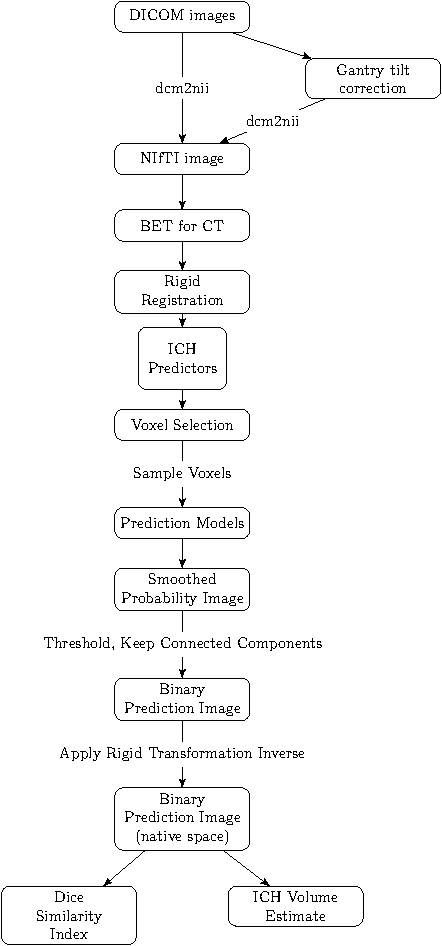
\includegraphics[width=0.5\linewidth]{Imaging_Pipeline_Flowchart_with_Rigid.pdf}
\caption{{\bf Processing Pipeline}.  Images in DICOM (Digital Imaging and Communications in Medicine) format were gantry tilt corrected if necessary and converted to NIfTI (Neuroimaging Informatics Technology Initiative) format using \texttt{dcm2nii}.  After NIfTI conversion, the brain extraction tool (BET) was applied to the image using a previously published protocol.  The image was rigidly registered to a brain CT template.  We estimated imaging predictors and used these predictors to estimate the probability of ICH in a prediction model.  The probability of ICH was thresholded, connected component below $100$ voxels ($0.1$mL) were discarded, and the image was transformed back into native space.  The ICH volume and the Dice Similarity Index, an overlap measure, were calculated compared to the true estimate from the manual segmentation.  }
\label{fig:framework}
\end{figure}

\subsection{Image Registration}
\citet{rorden_age-specific_2012} introduced a CT template based on $35$ individuals who presented with specific neurological deficits that were suspected to be caused by a stroke, but were later found to be due to a metabolic abnormality.  This CT template is represented in MNI (Montreal Neurological Institute) space and brain-extraction was performed on the template.  Prior to image processing, brain-extracted images were registered to this brain-extracted template using a rigid-body (6 degrees of freedom) and linearly interpolated to a $1\times1\times1$mm voxel resolution.  Transformed hemorrhage masks and brain masks were thresholded using a value of $0.5$. This operation reoriented the image, ensured isotropic voxel sizes for smoothing and other operations below, and preserved the relative volume of the ICH.  All image operations are done in MNI space, unless otherwise specified.


\subsection{Voxel Selection}
Each brain mask was eroded by a box kernel ($3mm\times3mm\times1$mm).  Though this erosion may exclude voxels from superficial bleeds towards the cortical surface, it excludes voxels with similar ranges as ICH voxels, caused by 1) incomplete skull stripping or 2) partial voluming effects with the skull.  If any voxels from the ICH mask was removed due to brain extraction or brain mask erosion, these voxels were included in estimating model performance but their predicted probability of ICH was set to $0$.  Therefore, these deleted ICH voxels will always be incorrectly predicted as not ICH.  

%This eroded mask and any excluded ICH voxels contained all voxels used for exploratory analysis and model fitting, which we will refer to as candidate voxels.



\subsection{Imaging Predictors}
We derived a set of imaging predictors from each CT scan.  We will describe each here with their rationale for use.  These features make up the potential set of predictors for image segmentation.
%Note that the corresponding images have roughly a distribution of between $0$ and $100$ HU as they have been skull stripped.  

\subsubsection{CT voxel intensity information} The raw voxel intensity value in HU was included, as it is the main predictor used in visual inspection; high HU values are indicative of hemorrhage. We created an indicator if the value was greater than $40$ and less than $80$ HU, similar to the criteria used for manual segmentation. 

\subsubsection{Local Moment Information} For each voxel, we extracted a neighborhood, denoted $N(v)$, of all adjacent neighboring voxels in $3$ dimensions and the voxel itself.  Let $x_k(v)$ denote the voxel intensity in HU for voxel neighbor $k$, where $k = 1, \dots, 27$.  We created the voxel neighborhood mean intensity ($\bar{x}(v)$):
\begin{equation}
\bar{x}(v) = \frac{1}{N(v)} \sum_{k \in N(v)} x_k(v) \label{eq:mean}
\end{equation}
We calculated the voxel neighborhood standard deviation (SD), skew, and kurtosis using the following method of moments estimators:
\begin{eqnarray*}
\text{SD}(v) &=& \sqrt{ \frac{1}{N(v)} \sum_{k \in N(v)} \left(x_k(v) - \bar{x}(v)\right)^2 } \\
\text{Skew}(v) &=& \frac{ \frac{1}{N(v)} \sum\limits_{k \in N(v)} (x_k(v)-\bar{x}(v) )^3 } {\left[ \frac{1}{N(v)} \sum\limits_{k \in N(v)} (x_k(v)- \bar{x}(v))^2\right]^{3/2}} \\
\text{Kurtosis}(v) &=& \frac{ \frac{1}{N(v)} \sum\limits_{k \in N(v)} (x_k(v)-\bar{x}(v) )^4 }{ \left( \frac{1}{N(v)} \sum\limits_{k \in N(v)} \left(x_k(v) - \bar{x}(v)\right)^2\right)^2} \\
\label{eq:moment}
\end{eqnarray*}
We acknowledge that we did not divide by $N(v) - 1$ for standard deviation and skewness, nor did we subtract by $3$ for kurtosis.  As $N(v)$ should be the same per voxel, this should not affect the estimates for prediction: it will be accounted for in any generalized linear model by the intercept and scaling of the beta coefficients and a tree-based decision algorithm will simply have a different cutoff value for binning.

Voxels higher in their local mean correspond to voxels adjacent to higher HU voxels on average, which are are more likely to be ICH.  The higher order moments can provide information about how homogeneous the intensities in the neighborhood are and where edges occur.  We also calculate the percentage of voxels in each neighborhood ($p_{\text{thresh}}(v)$) that have HU values between $40$ and $80$:
\begin{equation}
p_{\text{thresh}}(v) = \frac{1}{N(v)} \sum_{k \in N(v)} I\{ 40 \leq x_k(v) \leq 80 \} \label{eq:pct}
\end{equation}
which should be higher for ICH voxels as they are surrounded by high HU values.  

Voxels that are on the surface or surrounded by non-brain tissue as these are less likely to be ICH.  Voxels not within the the eroded mask are set to $0$, the following predictors assume that voxels close to many voxels with intensity $0$ are less likely to be ICH.    
We calculated the percentage of voxels that have neighbors of value of $0$:
\begin{equation}
p_{0}(v) = \frac{1}{N(v)} \sum_{k \in N(v)} I\{ x_k(v) = 0 \} \label{eq:pct0}
\end{equation}
and an indicator of whether any voxels in the neighborhood had a value of $0$:
\begin{equation}
\bar{I}_{0}(v) = I\{ p_{0}(v) > 0 \} \label{eq:I0}
\end{equation}
 
\subsubsection{Within-plane Standard Scores} Some brain structures have high HU values but are not ICH, such as the falx cerebri, which lies largely on the mid-sagittal plane.  Moreover, tissues in the top of the brain may have a higher average HU than those in the middle or bottom of the brain.  Thus, if values are standardized within each plane (axial, sagittal, coronal), these standard-plane scores may distinguish high values within a plane regardless of a mean shift, which may indicate ICH voxels.

We created standard-plane scores for each voxel on a slice-based level for axial, sagittal, and coronal planes. For each plane $o \in \{$axial, sagittal, and coronal$\}$, we calculated the standard-plane score as follows: 
\begin{equation}
z_{o}(v) = \frac{x(v) - \bar{x}(v, o)}{\sigma(v, o)} \label{eq:z}
\end{equation}
where $\bar{x}(v, o)$ and $\sigma(v, o)$ denote the mean and standard deviation of plane $o$ which contains voxel $v$, excluding voxels outside the brain mask.   In addition to the standardized images within plane we created a Winsorized standardized image, using the Winsorized mean and standard deviation, with a 20\% trimming of the distribution, which may allow for better standardization with artifacts of the distribution (such as gross hyperintensities). 

\subsubsection{First-pass Segmentation} We used a previously-published, open-source, general segmentation tool based on Markov random fields for image segmentation, called Atropos \citep{atropos}.  We used a 4-tissue class segmentation, and combined the top 2 probability values into one class.  We used this probability image as a predictor.  Although this tool has been shown to perform well in other studies for tissue-class segmentation, it did not perform adequately as a standalone segmentation tool for ICH in CT.  

\subsubsection{Contralateral Difference Images}  As most hemorrhages are constrained to one side of the brain, the contralateral side should have have lower HU values.  For non-hemorrhage voxels, however, the contralateral voxels would have similar HU values, and thus their difference would be small or negative.  Thus, we right-left flipped the image, and took a difference image: 
\begin{equation}
f(v) = x(v) - x(v^{*}) \label{eq:flip}
\end{equation}
where $v^{*}$ is the voxel from the contralateral side.  



\subsubsection{Global Head Information} We used the distance to the brain centroid ($d(v)$) to potentially down-weight voxels that are very far from the brain center, which may be artifacts.    We also created $3$ images which were obtained by smoothing the original image using large Gaussian kernels ($\sigma = 5mm^3, 10mm^3, 20mm^3$), which can capture any potential homogeneity throughout the scan, denoted by $s_{5}(v)$, $s_{10}(v)$ and $s_{20}(v)$, respectively.   

\subsubsection{Standardized-to-template Intensity}  
Although standardizing voxels compared to within-scan measurements can detect anomalous tissue, one powerful tool is to use a measure how different a voxel is compared to that voxel in a person from a non-stroke population.  We registered the brain-extracted image to the brain-extracted CT template using an affine transformation, followed by a non-linear transformation estimated using Symmetric Normalization (SyN) \citep{avants_symmetric_2008}.  
From $30$ CT images from non-stroke patients from Dr.~Rorden (personal communication), we registered these non-stroke, brain-extracted scans to the CT template, and created a voxel-wise mean image $M$ and voxel-wise standard deviation $S$ image in template space.  For each scan in our study, we created a standardized voxel intensity with respect to this population ($z_{\text{template}}$) using the following equation:
$$
z_{\text{template}}(v) = \frac{x(v) - M(v)}{S(v)}
$$
This image is warped back into the rigid-body-registered space so that these standardized voxels are aligned with other predictors.  This predictor is similar to that used in \citet{gillebert_automated_2014}.  



%To further illustrate how smoothing affects brain extraction, we present one example case where brain extraction performance with BET was acceptable only after smoothing.  




\subsection{Model Creation}
We chose 10 scans from 10 patients to perform exploratory data analysis, model fitting, and estimation of model cutoffs, denoted as training data. Of the 102 remaining scans, we split the data into $51$ validation scans and  $51$ test scans.  


From the training data we estimated the $0.5\%$ and $99.5\%$ quantiles for all ICH voxels in the predictors.  Voxels that were jointly within these quantiles for $z_{\text{axial}}$, $z_{\text{coronal}}$, $p_{\text{thresh}}$, and within HU between $30$ and $100$ were considered candidate voxels of ICH; voxels outside of the intersection of these ranges were given a $0$ probability of ICH. These cutoffs empirically found to be robust in the test scans, they excluded a mean 63.6 (min: 37.1, max: 89.8) percentage of non-ICH voxels, while including a mean 97.9 (min: 91.6, max: 99.9) percentage of ICH voxels.  This voxel-selection procedure should improve the specificity of model predictions, and improve computational speed.   All models were fit with all predictors.  

From these 10 scans, we collapsed all the voxels passing the voxel selection procedure.  From these voxels, we randomly sampled  100,000 to fit the models and do data exploration, and used the remaining voxels to estimate the model cutoffs of the probability of ICH.

% get Reseg_Aggregate_data Rda for nunmber of voxels 


\subsection{Models}

Using the sampled training voxels, we created predictions for the probability of ICH using a 1) logistic regression model, 2) logistic regression model with the LASSO  penalty, 3) generalized additive model (GAM), and 4) classifier fit with the random forest algorithm.

For the standard and penalized logistic regression model, we used all predictors.  The penalized model was fit using the LASSO (Least Absolute Shrinkage and Selection Operator) penalty \citep{tibshirani_regression_1996} using the \pkg{glmnet} package \citep{friedman_regularization_2010}.  The tuning parameter ($\lambda$) for the penalization was chosen using 10-fold cross-validation (of only the training voxels), with the cost function of misclassification rate.  The parameter was chosen using the largest value such that the error is within 1 standard error of the minimum, chosen for out-of-sample performance stability.

The generalized additive model (GAM) \citep{hastie_generalized_1986, hastie_generalized_1990} was also created using indicator variables for binary variables and thin-plate splines for all continuous measures, fit with fast-estimation of restricted maximum likelihood (fREML) using the \pkg{mgcv} package \citep{wood_fast_2011, wood_generalized_2015}.  


We fit a random forest \citep{breiman2001random} using the \pkg{randomForest} package in R \citep{randomForest}, using the default pruning parameters and number of trees (\verb|ntree|=500, \verb|mtry|=4). 



\subsection{Estimating a Cutoff for Model Probability}

Each model gives the estimate of the probability a voxel is ICH.  In the end, however, we would like a binary prediction mask to compare to the manual segmentation. 
Using the voxels from the training data, we estimated the probability of ICH from each model.  For each model probability, we smoothed this probability image using the neighborhood voxels (1 voxel in every direction).  To choose a probability cutoff to make a binary image, we used the voxels in the training data that were not sampled for estimating the model.  Using these voxels in the smoothed images, we estimated the probability cutoff that minimized the Dice Similarity Index (DSI) \citep{dice_measures_1945} between the prediction and true value.   The DSI is measure of overlap insensitive to values where neither the true segmentation or predicted segmentation were considered ICH, and will be used as a performance measure when comparing models.

After thresholding the smoothed image using this probability cutoff, we discarded regions with fewer than 100 ($0.1$ milliliters) connected voxels.  We then transformed this binary mask back to native space using the inverse from the previously-estimated rigid-body transformation.  As the linear interpolation results in a non-binary mask, we thresholded this image at $0.5$ to preserve volume \cite{flirt_reg}.  

For each scan in the validation data, this prediction process was performed and each each scan has a corresponding binary prediction  image.


\subsection{Measuring and Testing ICH Prediction Performance}

For all measures, we used the binary prediction masks from the validation scans.  We measured performance for each model using the DSI and also estimated the ICH volume of the prediction. Specificity and overall accuracy are inflated by the fact that most of the voxels within the brain are non-ICH.  We also calculated the relationship of estimated volume of ICH compared to the manual segmentation using the Pearson correlation and root mean squared (RMSE) between volumes measures. For DSI and correlation, higher values indicate better agreement with the manual segmentation.  For RMSE, lower indicates better agreement.


\section{Results}

\subsection{Dice Similarity Index}

In Figure~\ref{fig:dice}, we show the DSI distributions from the validation data for each model.  We see that DSI is high on average for all models, with a few scans having a very small DSI (i.e. failures).   The median DSI for each model was: $0.89$ (logistic), $0.885$  (LASSO), $0.88$ (GAM), and $0.899$ (random forest). 
We also note that using the random forest results in a slightly higher median DSI compared to the other models.  Overall, the results indicate good overlap between the predicted ICH segmentation and manual ICH segmentation. 





\subsection{ICH Volume Estimation}
In Figure~\ref{fig:vol}, we show the estimated ICH volume versus that from the manual segmentation.  The pink line represents the $X = Y$ line, where the estimated and true volume are identical.  The blue line represents the linear fit; the line equation and correlation are printed on the plot.  The farther away the slope of the equation is from $1$ represents a multiplicative bias, where values greater than $1$ represents larger estimated volumes.  The farther the intercept is from $0$ represents and additive bias in the estimated volume, where values greater than $0$ again represent larger estimated volumes.  The correlation (95\% confidence interval (CI)) between the true volume and the volume predicted volume were $0.92$ (95\% CI: $0.884, 0.945$ for the logistic model, 
$0.916$ ($0.878, 0.942$) for the LASSO, 
$0.908$ (95\% CI: $0.866, 0.937$) for the GAM, and  
$0.932$ (95\% CI: $0.901, 0.954$) for the random forest. 

\subsection{Model Choice}
Overall, all models perform adequately for ICH segmentation.  Some failures exist, but the algorithm using the 





\begin{figure}
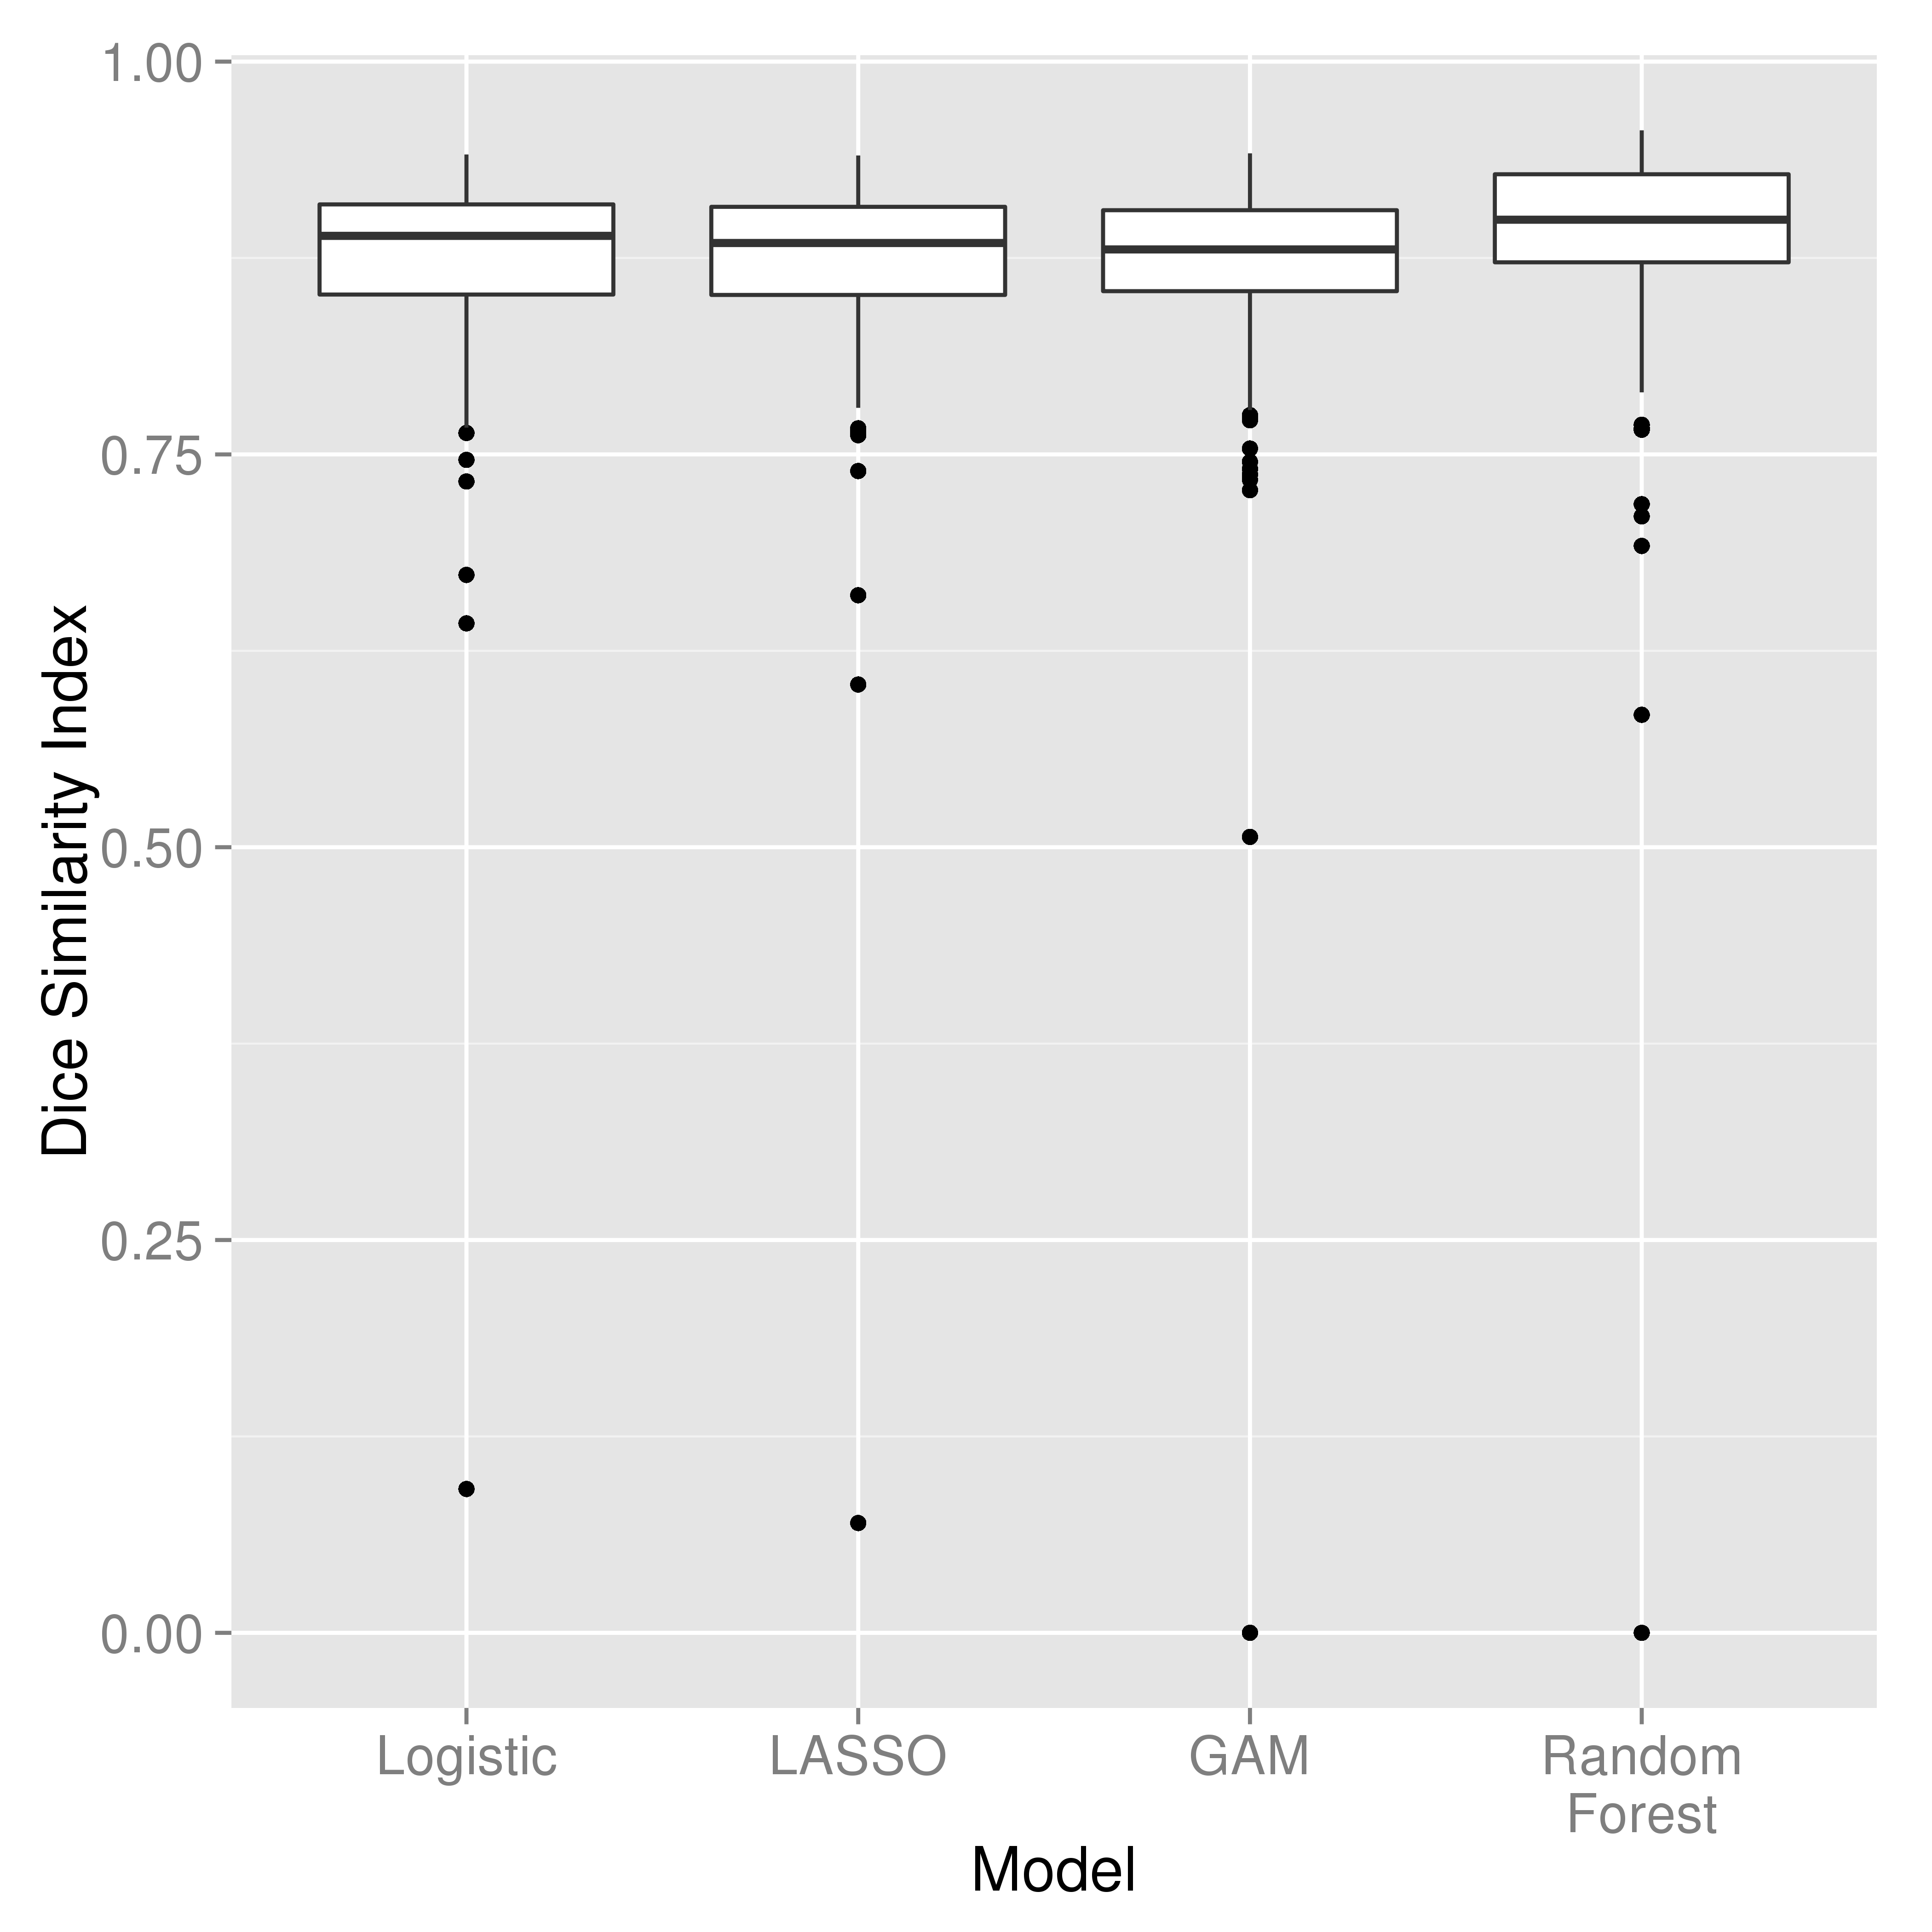
\includegraphics[scale=1]{Reseg_Dice_Comparison.png}
\caption{{\bf Distribution of Dice Similarity I} }
\label{fig:dice}
\end{figure}

\begin{figure}
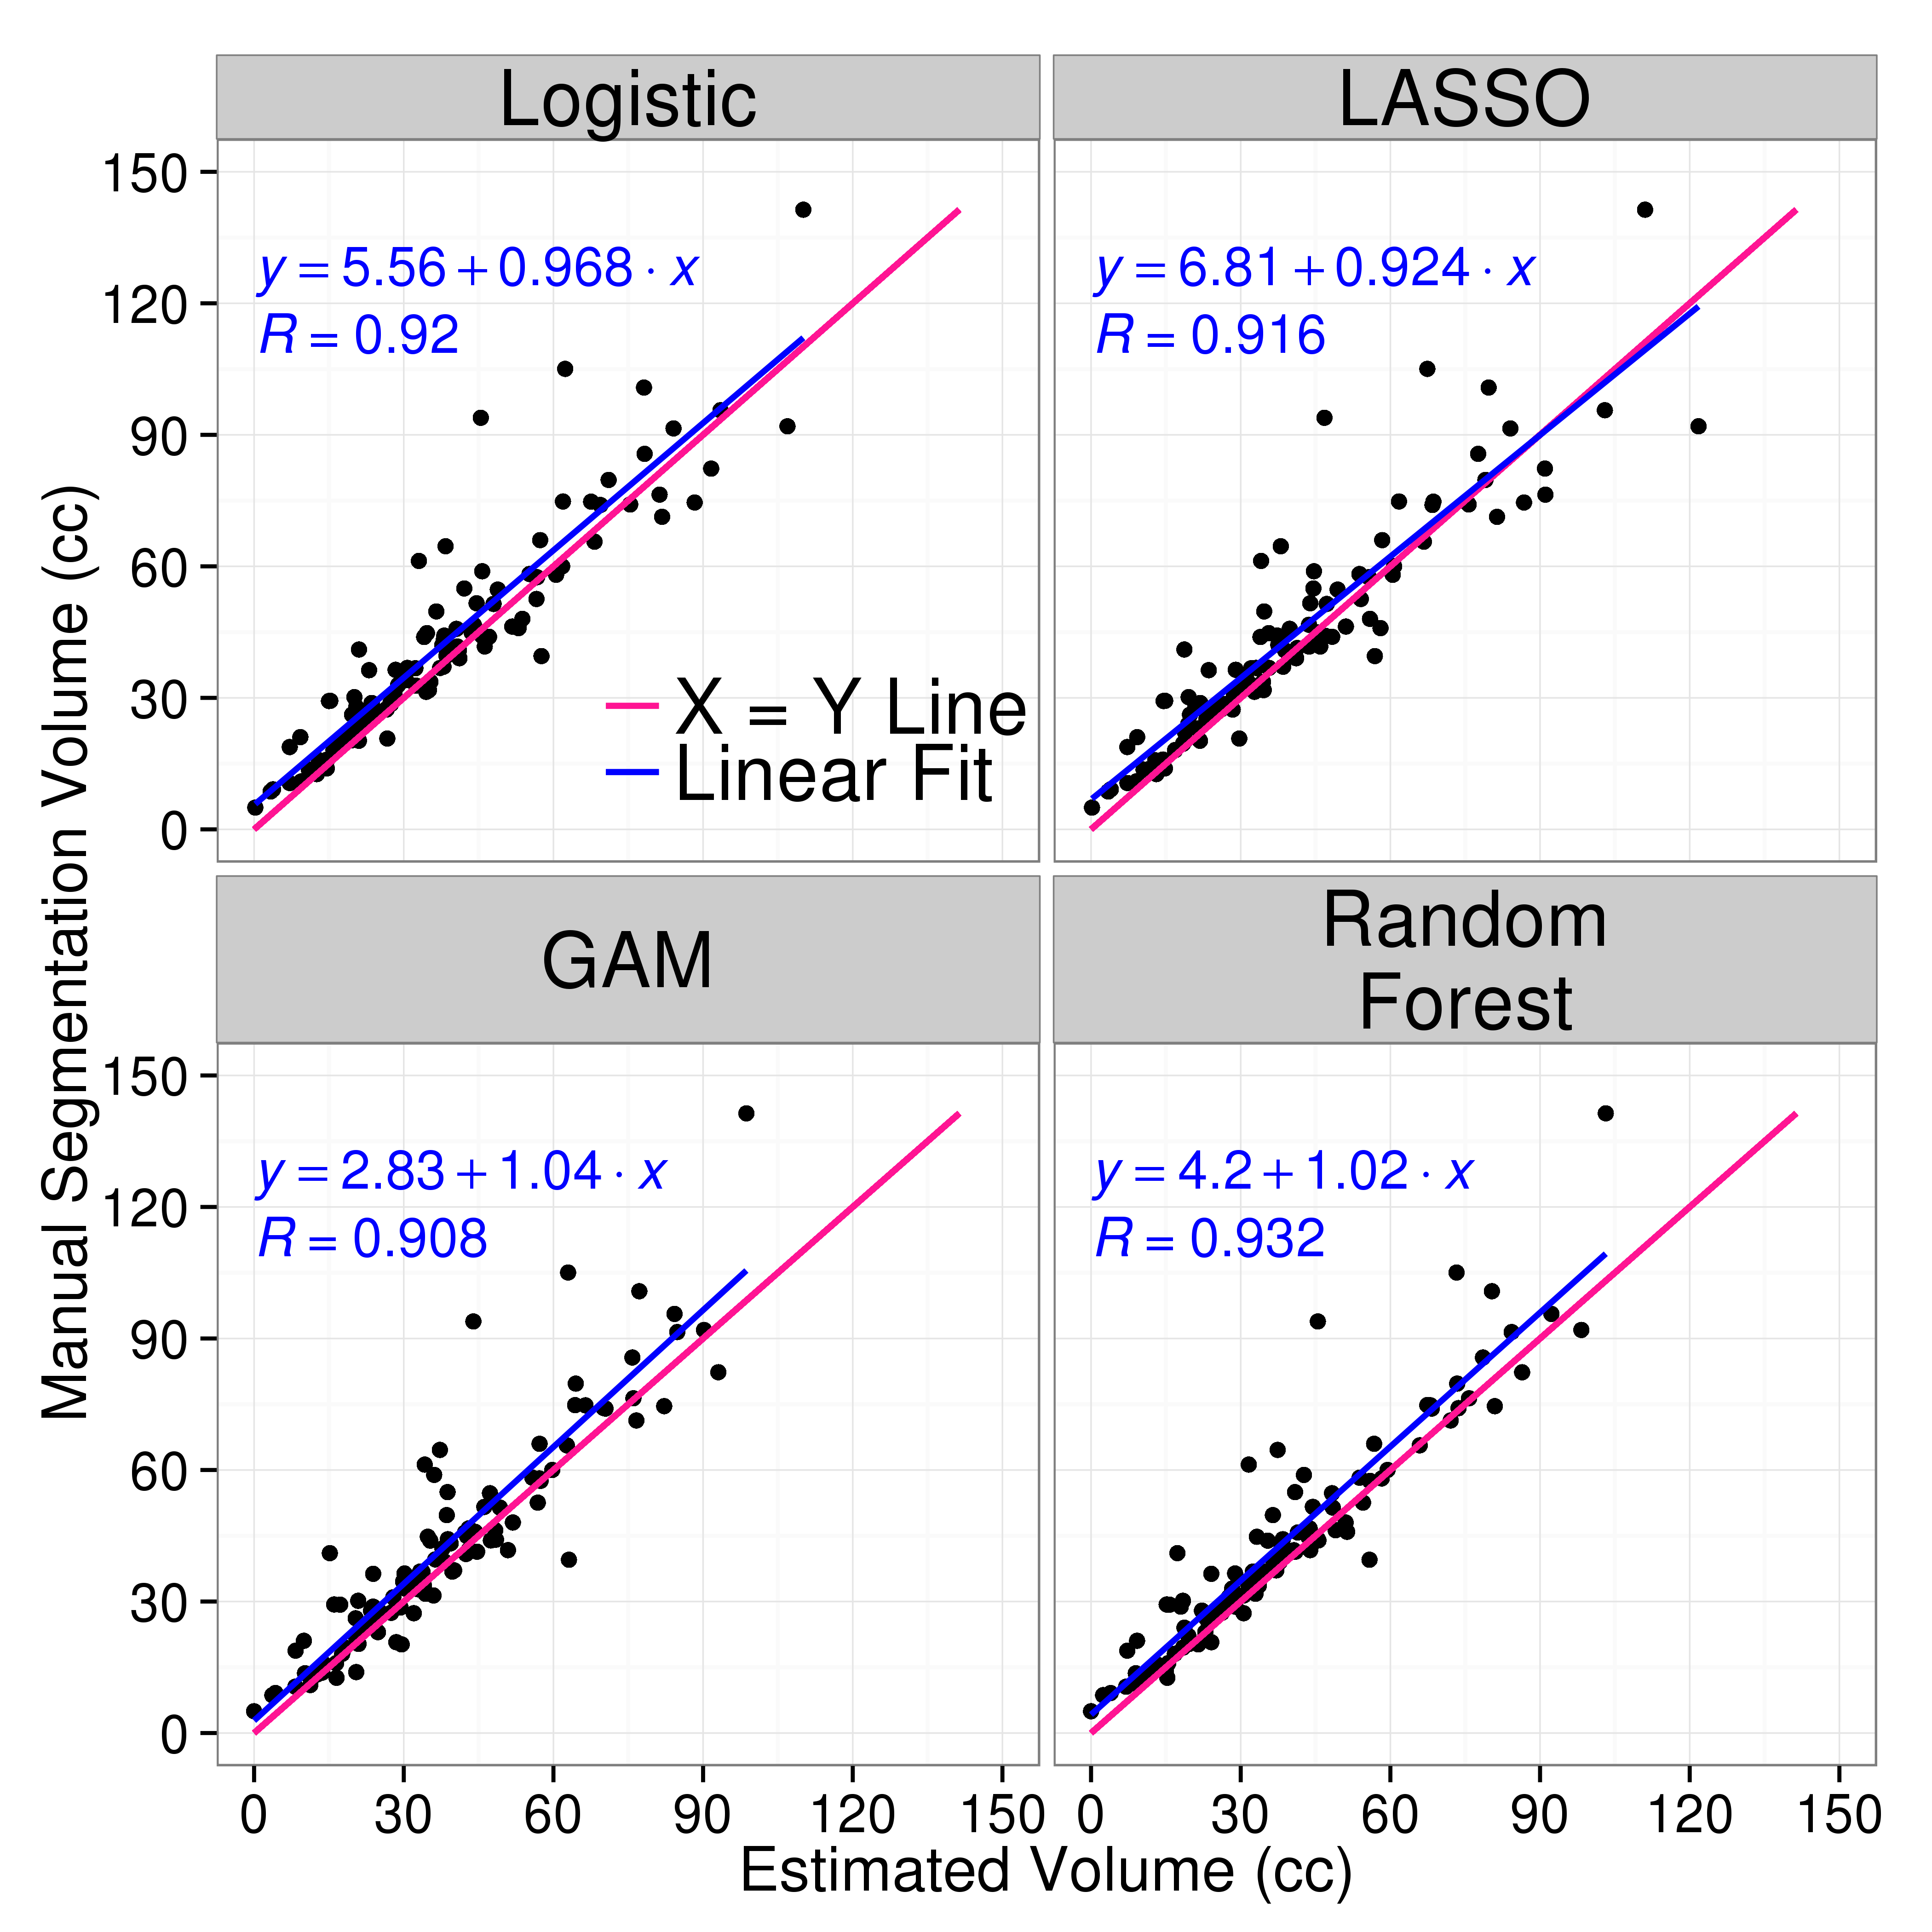
\includegraphics[scale=1]{Reseg_Volume_Comparison.png}
\caption{}
\label{fig:vol}
\end{figure}


\section{Discussion}

We have presented a fully automated of hemorrhage segmentation for intracranial hemorrhage.  We create a set of predictors that attempt to capture the features relevant to distinguishing ICH versus non-ICH areas.
The models use allow for a relatively fast and intuitive estimation of the probability of ICH.  We have incorporated different aspects of a CT scan, each representing intuitive information.  Different pipelines were used to determine which processing methods could potentially improve ICH prediction.



\section*{Acknowledgments}
We thank the patients and families who volunteered for this study and Genentech Inc. for the donation of the study drug (Alteplase).

\section*{Sources of Funding}
The project described was supported by the NIH grant RO1EB012547 from the National Institute of Biomedical Imaging And Bioengineering, T32AG000247 from the National Institute on Aging, R01NS046309, RO1NS060910, RO1NS085211, R01NS046309, U01NS080824 and U01NS062851 from the National Institute of Neurological Disorders and Stroke, and RO1MH095836 from the National Institute of Mental Health. Minimally Invasive Surgery and rt-PA in ICH Evacuation Phase II (MISTIE II) was supported by grants R01NS046309 and U01NS062851 awarded to Dr. Daniel Hanley from the National Institutes of Health (NIH)/National Institute of Neurological Disorders and Stroke (NINDS).  ICES was led by Co-Principal Investigator Dr. Paul Vespa at the University of California Los Angeles. Minimally Invasive Surgery and rt-PA in ICH Evacuation Phase III (MISTIE III) is supported by the grant U01 NS080824 awarded to Dr. Daniel Hanley from the National Institutes of Health (NIH)/National Institute of Neurological Disorders and Stroke (NINDS). Clot Lysis: Evaluating Accelerated Resolution of Intraventricular Hemorrhage Phase III (CLEAR III) is supported by the grant U01 NS062851 awarded to Dr. Daniel Hanley from the National Institutes of Health (NIH)/National Institute of Neurological Disorders and Stroke (NINDS). 

\newpage
%\section*{References}
%\bibliographystyle{elsarticle-num-names}
%\bibliography{CT_ICH_Segmentation}
%\bibliography{CT_Skull_Stripping_Bib}
\printbibliography

\section{Appendix}

\subsection{Model Specification}


Let $Y_{i}(v)$ represent the binary hemorrhage mask indicator for voxel $v$, from patient $i$, and $x_{i,v}(k)$ represent the predictor image for image $k$, $k = 1, \dots 21$.
$$
\text{logit}\left(P(Y_{i}(v) = 1)\right) = \beta_0 + \sum_{k = 1}^{21} x_{i, k}(v)\beta_{k}
$$

The coefficients for the logistic model are (in log odds or log odds ratios):

% latex table generated in R 3.2.2 by xtable 1.8-0 package
% Tue Jan 19 15:41:05 2016
\begin{table}[ht]
\centering
\begin{tabular}{lr}
  \hline
term & estimate \\ 
  \hline
Intercept & 1.0077 \\ 
  Neighborhood mean & 0.0514 \\ 
  Neighborhood sd & 0.0001 \\ 
  Neighborhood skew & 0.0650 \\ 
  Neighborhood kurtosis & -0.3515 \\ 
  Image intensity (HU) & -0.1723 \\ 
  Threshold ($>$= 40 and $<$= 80) & -0.1514 \\ 
  Z-score plane 1 & -0.6322 \\ 
  Z-score plane 2 & -0.2493 \\ 
  Z-score plane 3 & 1.0369 \\ 
  Winsorized z-score (20$\backslash$\% trim) & 0.5475 \\ 
  Percentage thresholded neighbors & 2.0612 \\ 
  Atropos probability image & 0.1497 \\ 
  Percent of zero neighbors & -9.1802 \\ 
  Indicator of any zero neighbors & 0.0708 \\ 
  Distance to Image centroid & -0.0870 \\ 
  Gaussian smooth (5mm\verb|^|3) & -0.0507 \\ 
  Gaussian smooth (10mm\verb|^|3) & 0.5499 \\ 
  Gaussian smooth (20mm\verb|^|3) & -0.3897 \\ 
  Z-score-to-template image & 1.4598 \\ 
  Contralateral difference & 0.0326 \\ 
   \hline
\end{tabular}
\end{table}


The specification for the functional form of the model fit with the LASSO penalty, is the same, but optimizes the following criteria:
$$
\min_{\beta} - \left( \frac{1}{\sum_{i}V_i} \sum_i Y_{i}(v) \times X_i(v)\beta - \log \left(1 + e^{X_i(v)\beta}\right) \right) +\lambda\sum_{k}\left|\beta_k\right|
$$



\end{document}


\newpage
\singlespacing
\section{Outline}
\begin{enumerate}
\item Introduction
	\begin{enumerate}
	\item Why is ours better? 
	\begin{enumerate}
		\item Fast (at computation but not making predictors)
		\item 3D - many applications show only in 2D on a slice.  
		\item Fully automated - not semi-automated
	\end{enumerate}
	\end{enumerate}
\item Methods
	\begin{enumerate}
	\item Data (MISTIE), CT info (non-contrast), and Preprocessing
	\begin{enumerate}
		\item Need resolution of data 5mm vs 1mm and total volume of hemorrhage and varslice
		\item Problem with varslice and registration - need interpolation - rerun without for sensitivity analysis?
	\end{enumerate}
	\item Imaging Predictors
	\begin{enumerate}
		\item If we use SyN, why not use that as a reg tool?
		\item Mean and SD images are from Rorden - need permission and also maybe get an independent dataset
		\item DO WE NEED THESE FOR SPECIFICITY? - can use the OSiriX or the post-scans
		\begin{enumerate}
			\item Can also give an indicator of ANY hemorrhage or not.  
		\end{enumerate}
		\item Also - use his normalization to the template and compare mean/sd images vs. SyN.
		\begin{enumerate}
			\item This will be important based on the skull-stripping of the template image.
		\end{enumerate}
	\end{enumerate}
	\item Logistic Models - Model Selection
	\item Performance Criteria - Sensitivity, Accuracy, Dice, pAUC, Volume Estimation (talk about varslice)
	\begin{enumerate}
		\item If we say Volume estimation is the most important, why not just use that 	
		\item Sensitivity can be about localization/IVH engagement.  Need fixed Specificity
		\item pAUC - good tradeoff between sensitivity and specificity, but have low sensitivity 
		\item Accuracy is plagued by large number of 0s
		\item Sensitivity with fixed specificity.  Trade off some specificity (reasonable) for a good sensitivity (larger than accuracy).
	\end{enumerate}
	\item Describe how for each criteria, we will present the ``best'' model for each.  
	\end{enumerate}
\item Results
	\begin{enumerate}
	\item How to present different ``best'' models for different criteria.
	\item From the ``best'' model, take out subsets of predictors to see how it improves the cost function (pAUC, sens, etc).
	\end{enumerate}
\item Discussion
	\begin{enumerate}
	\item Not Perfect segmentation, but good enough for certain tasks.
	\item registration to template from rorden smooths the hemorrhage mask, so if masked out when smoothed, then OK
	\item Different cost functions
	\item Cutoffs worked for large number of different scans
	\item May need to show a per scanner comparison.  
	\item Needs to be implemented on Shiny Server (Ask Adi)
	\item Relies on a good Skull stripping.  Need to do update my GitHub page for this - especially the fixes for large scans.
	\end{enumerate}
\item Conclusion
	\begin{enumerate}
	\item We can do segmentation - what about SOFTWARE?
	\item Don't need to release batch processing if on smart stats
	\item This can be after the paper
	\end{enumerate}
\item Figures
	\begin{enumerate}
		\item Processing Pipeline
		\item Skull Stripped image, with Erosion
		\item Predictor image - those that worked the best - union of all selected, Candidate voxel image
		\item 3-4 different patients with ROI and prediction.  Show good AND bad.
		\item ROC Curve of dropping out predictors 
		\item Population based ROC curve - or just on sampled data?
		\item Computation time?
	\end{enumerate}
\end{enumerate}

\section{Questions?}
\begin{enumerate}
\item What else is out there?  How to get our data analyzed by that data for comparison?
\item What papers to read?
\item Are all these non-contrast scans? Ask Andrew what protocol states
\item What does Dan think is the most important measure?  If none, can we use them all?
\item What do we need to release?  Let's talk to Adi ASAP.
\item Email seg paper from previous (Bhanu)
\item What about IP here?  How to get that rolling?
\item Comparison to ABC/2?
\end{enumerate}






